\begin{figure*}[t]
\centering
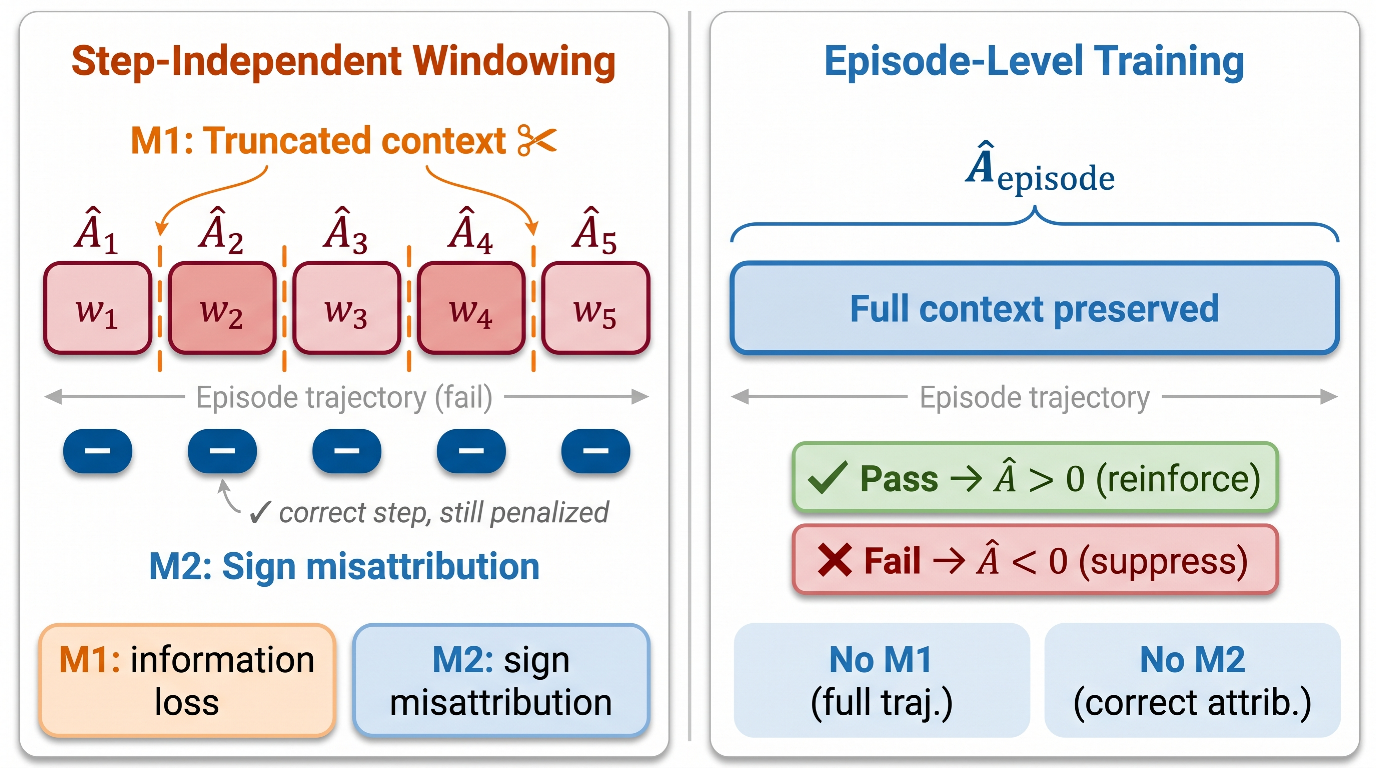
\includegraphics[width=0.85\textwidth]{fig_overview.pdf}
\caption{Step-independent windowing (left) partitions the trajectory into fixed windows, each optimized independently. This introduces two failure mechanisms: M1 (information loss) truncates context at window boundaries, and M2 (sign misattribution) assigns all windows the same advantage sign based on episode outcome. Episode-level training (right) treats the full trajectory as a single sample, eliminating both mechanisms.}
\label{fig:overview}
\end{figure*}

\section{Introduction}
\label{sec:introduction}

Reinforcement learning from sparse terminal reward has emerged as a promising paradigm for training LLM agents on multi-turn interactive tasks spanning 30--50 interaction steps~\citep{kim2025reflact,digiRL2024,wang2022scienceworld}. Group Relative Policy Optimization (GRPO)~\citep{shao2024deepseekmath}, with its critic-free design, has become the algorithm of choice. Yet a gap persists between the promise of RL-driven agent improvement and the reality of training outcomes: recent agent RL systems~\citep{ragen2025,selfguide2026,spear2025,feng2025gigpo} share a common, unscrutinized implementation pattern (decomposing trajectories into fixed-size windows, each optimized independently) and frequently report training instability without diagnosing its root cause.

We show this \textit{step-independent} default introduces a fundamental credit assignment pathology. Step-independent training partitions trajectories into non-overlapping $h$-step windows, each optimized via GRPO. This produces a two-phase collapse: task success drops to 0\% while action validity initially remains high, then continued training destroys even basic formatting. Preliminary comparisons suggest that standard remedies (dense reward shaping, discount tuning) do not resolve the pathology (Appendix~\ref{app:additional}). Concurrent methods that improve per-step credit quality (GiGPO~\citep{feng2025gigpo}, GAGPO~\citep{gagpo2026}, Turn-PPO~\citep{turnppo2025}, HCAPO~\citep{hcapo2026}) address the credit assignment challenge through improved step-level mechanisms, validating that sign correctness is the critical factor. Our contribution is orthogonal: we formally diagnose \textit{why} the default windowing fails.

We trace the collapse to two mechanisms at different layers. \textit{\textbf{Policy information loss}} (M1) operates at the inference layer: each window lacks access to earlier observations, imposing a constant performance ceiling. \textit{\textbf{Advantage sign misattribution}} (M2) operates at the training layer: under binary reward, the advantage sign reflects episode success rather than local action quality. Our theoretical analysis shows that a substantial fraction of gradient updates for locally correct actions (those contributing to episode success; Definition~1) carry incorrect sign (Section~\ref{sec:theory}), a prediction confirmed by direct measurement (Section~\ref{sec:sign_verification}). Sign errors, amplified by the M1--M2 feedback loop, cause progressive degradation rather than merely slow convergence. Our primary contribution is diagnostic: we identify, formalize, and empirically validate a previously uncharacterized pathology in the dominant training paradigm. Episode-level GRPO (restoring GRPO's original per-sample granularity to the episode level) structurally eliminates both mechanisms by treating the full trajectory as a single optimization sample, achieving substantial OOD improvement where step-independent collapses to 0\%, with preliminary evidence of persistence at 8B scale.

Our contributions:
\begin{enumerate}[nosep,leftmargin=*]
\item \textbf{Dual mechanism diagnosis.} We formalize \textit{information loss} and \textit{sign misattribution} as distinct failure modes with different temporal behaviors (constant ceiling versus cumulative degradation) and derive closed-form expressions for the probability of incorrect gradient direction.
\item \textbf{Controlled empirical separation.} A partial factorial experiment isolates each mechanism: removing sign misattribution converts collapse into bounded learning; removing information loss enables OOD generalization. Direct sign measurement confirms the theoretical prediction at near-random credit agreement (alignment between advantage sign and action quality).
\item \textbf{Systematic evaluation and generality.} Episode-level training structurally eliminates both mechanisms, but an 11-seed evaluation reveals that avoiding collapse is necessary but not sufficient: only 36\% of seeds achieve significant OOD transfer. Cross-scale (8B) and cross-environment (ScienceWorld) evidence provides preliminary support for generality.
\end{enumerate}
